% \documentclass[russian,14pt,floatsection,nocolumnsxix, nocolumnxxxii,nocolumnxxxi]{eskdtext}
\usepackage[utf8x]{inputenc}

% закомментировать для рамок 
\usepackage[numbertop, numbercenter]{eskdplain}

% для объединения строк в таблице
\usepackage{multirow}



% для размера колонок
\usepackage{tabularx}
\usepackage{lscape}
\newcolumntype{n}{>{\hsize=.4\hsize}X}
\newcolumntype{m}{>{\hsize=.2\hsize}X}


\usepackage{setspace}
\onehalfspacing % полуторный интервал для всего текста

% - Подключаем шрифты из пакета scalable-cyrfonts-tex
\usepackage{cyrtimes}

% - Отступ красной строки
\setlength{\parindent}{1.25cm}

% - Убирает точку в списке литературы
\makeatletter
\def\@biblabel#1{#1 }

% ограничение для оглавления
%\usepackage{tocvsec2}
\setcounter{tocdepth}{2}

% - Точки для всех пунктов в оглавлении
\renewcommand*{\l@section}{\@dottedtocline{1}{1.5em}{2.3em}}
\renewcommand*{\l@subsection}{\@dottedtocline{1}{1.5em}{2.3em}}
% \renewcommand*{\l@subsubsection}{\@dottedtocline{1}{1.5em}{2.3em}}

% - Для переопределения списков
\renewcommand{\theenumi}{\arabic{enumi}}
\renewcommand{\labelenumi}{\theenumi)}
\makeatother

\usepackage{enumitem}
\setlist{nolistsep, itemsep=0.3cm,parsep=0pt}

% - ГОСТ списка литературы
\bibliographystyle{utf8gost705u}


% - Верикальные отступы заголовков 
\ESKDsectSkip{section}{1em}{1em}
\ESKDsectSkip{subsection}{1em}{1em}
\ESKDsectSkip{subsubsection}{1em}{1em}

% - Изменение заголовков
\usepackage{titlesec}
\titleformat{\section}{\normalfont\normalsize\centering}{\thesection}{1.0em}{}
\titleformat{\subsection}{\normalfont\normalsize\centering}{\thesubsection}{1.0em}{}
\titleformat{\subsubsection}{\normalfont\normalsize\centering}{\thesubsubsection}{1.0em}{}
\titleformat{\paragraph}{\normalfont\normalsize\centering}{\theparagraph}{1.0em}{}

% - Оставим место под ТЗ 
\setcounter{page}{1}

% - Для больших таблиц
\usepackage{longtable}
\usepackage{tabularx}
\renewcommand{\thetable}{\thesection.\arabic{table}}

% - Используем графику в документе
\usepackage{graphicx}
\graphicspath{{images/}}
\renewcommand{\thefigure}{\thesection.\arabic{figure}}
% to have figure on top
%
\makeatletter
\setlength{\@fptop}{0pt}
\makeatother

% - Счётчики
\usepackage{eskdtotal}

% - Выравнивание по ширине
\sloppy

% - Разрешить перенос двух последних букв слова
\righthyphenmin=2

% - Оформление списков
\RequirePackage{enumitem}
\renewcommand{\alph}[1]{\asbuk{#1}}
\setlist{nolistsep}
\setitemize[1]{label=--, fullwidth, itemindent=\parindent, 
  listparindent=\parindent}% для дефисного списка
\setitemize[2]{label=--, fullwidth, itemindent=\parindent, 
  listparindent=\parindent, leftmargin=\parindent}
\setenumerate[1]{label=\arabic*), fullwidth, itemindent=\parindent, 
  listparindent=\parindent}% для нумерованного списка
\setenumerate[2]{label=\alph*), fullwidth, itemindent=\parindent, 
  listparindent=\parindent, leftmargin=\parindent}% для списка 2-ой ступени, который будет нумероваться а), б) и т.д.
  
% - Оформляем листинг кода (не использовать комментарии на русском!)
\usepackage{listings}  
\lstset{basicstyle=\ttfamily\scriptsize}
\lstset{extendedchars=\true}

% - выводим текст как есть с размером шрифта scriptsize
\makeatletter
\def\verbatim{\scriptsize\@verbatim \frenchspacing\@vobeyspaces \@xverbatim}
\makeatother

% - Вставка pdf
\usepackage[enable-survey]{pdfpages}

%межстрочный интервал
\usepackage{setspace}
\linespread{1.5}

%фамилии для рамок
\author{\ESKDfontII Мейта М.В.}
\ESKDchecker{\ESKDfontII Глухарева С.В.}
\ESKDnormContr{\ESKDfontII Якимук А.Ю.}
\ESKDapprovedBy{\ESKDfontII Шелупанов А.А.}
\ESKDcolumnI{\ESKDfontIII Технико-экономическое обоснование дипломной работы}
\ESKDcolumnIX{\ESKDfontIII ТУСУР, ФБ, каф.~КИБЭВС, гр.~722}
\ESKDsignature{КИБЭВС.58.29.29 ПЗ}

% 
% \begin{document}
%  
% 

\ESKDstyle{formIIab}
\ESKDputOnStyle{formII}{frame}{\renewcommand{\ESKDchecker}{\ESKDfontII Глухарева С.В.}}
\ESKDthisStyle{formII}

\renewcommand{\ESKDcolumnI}{\ESKDfontIII Технико-экономическое обоснование дипломной работы}


\section{Технико-экономическое обоснование дипломной работы}
\subsection{Обоснование актуальности дипломной работы}

Вследствие активного развития информационных технологий возрастает и количество преступлений в информационной сфере.
Зачастую злоумышленники, как внешние, так и внутренние, используют самостоятельно разработанные программы для осуществления 
атак на информационные ресурсы.
Системы, способные идентифицировать разработчиков вредоносного ПО, могут внести существенный вклад в развитие компьютерной
криминалистики, а также оказывать помощь в исследовании вопросов интеллектуальной собственности среди разработчиков программного
обеспечения.

Цель настроящей дипломной работы --- разработать ПО, способное идентифицировать автора программы по исходному коду, с перспективой его
дальнейшего применения в борьбе с киберпреступностью, в области лицензионных, патентных, и иных судебных разбирательств.


\subsection{Организация и планирование работы}

Основные задачи организации и планирования работ:
\begin{itemize}
 \item определение объема предстоящих работ;
 \item определение основных этапов работ;
 \item установление сроков выполнения запланированных работ;
 \item определение необходимых денежных, материальных и трудовых ресурсов.
\end{itemize}


При выполнении дипломной работы были задействованы следующие лица:
\begin{itemize}
 \item руководитель (рук.);
 \item исполнитель (исп.).
\end{itemize}

Студенты, не имеющие высшего образования, могут быть приняты на
работу техниками. Должностной оклад техника составляет 4400 рублей.
Стоимость одного часа работ равна 27,5 рублей.
Стоимость одного часа работ руководителя с ученой степенью кандидата наук и должностью доцента
согласно коллективному договору на 2016-2019 годы~\cite{kollectiv}
равна 230 рублей.   

Руководитель работы оказывает помощь исполнителю в планировании работ в период проектирования, рекомендует
необходимую литературу, проводит консультации, осуществляет контроль над выполнением всех 
намеченных этапов работы. Исполнитель реализует объем работ, установленный в техническом задании.

Для процесса дипломирования были определены следующие этапы:
\begin{enumerate}
 \item обзор информационных источников;
 \item моделирование;
 \item программная реализация разработанной модели;
 \item разработка программного интерфейса;
 \item сбор и обработка тестовых данных;
 \item тестирование и отладка полученной модели;
 \item анализ результатов;
 \item проведение расчетов по технико-экономическому обоснованию;
 \item проведение расчетов по безопасности жизнедеятельности;
 \item оформление, проверка и исправление пояснительной записки;
 \item подготовка необходимой документации;
 \item защита ВКР.
\end{enumerate}


Согласно выделенным этапам строится диаграмма
Ганта, отображающего затраты времени на выполнение проекта всеми
участниками (табл.~\ref{tab:job_is_done_2}).


\begin{table}[!ht]
\caption{График выполнения работ}
\centering
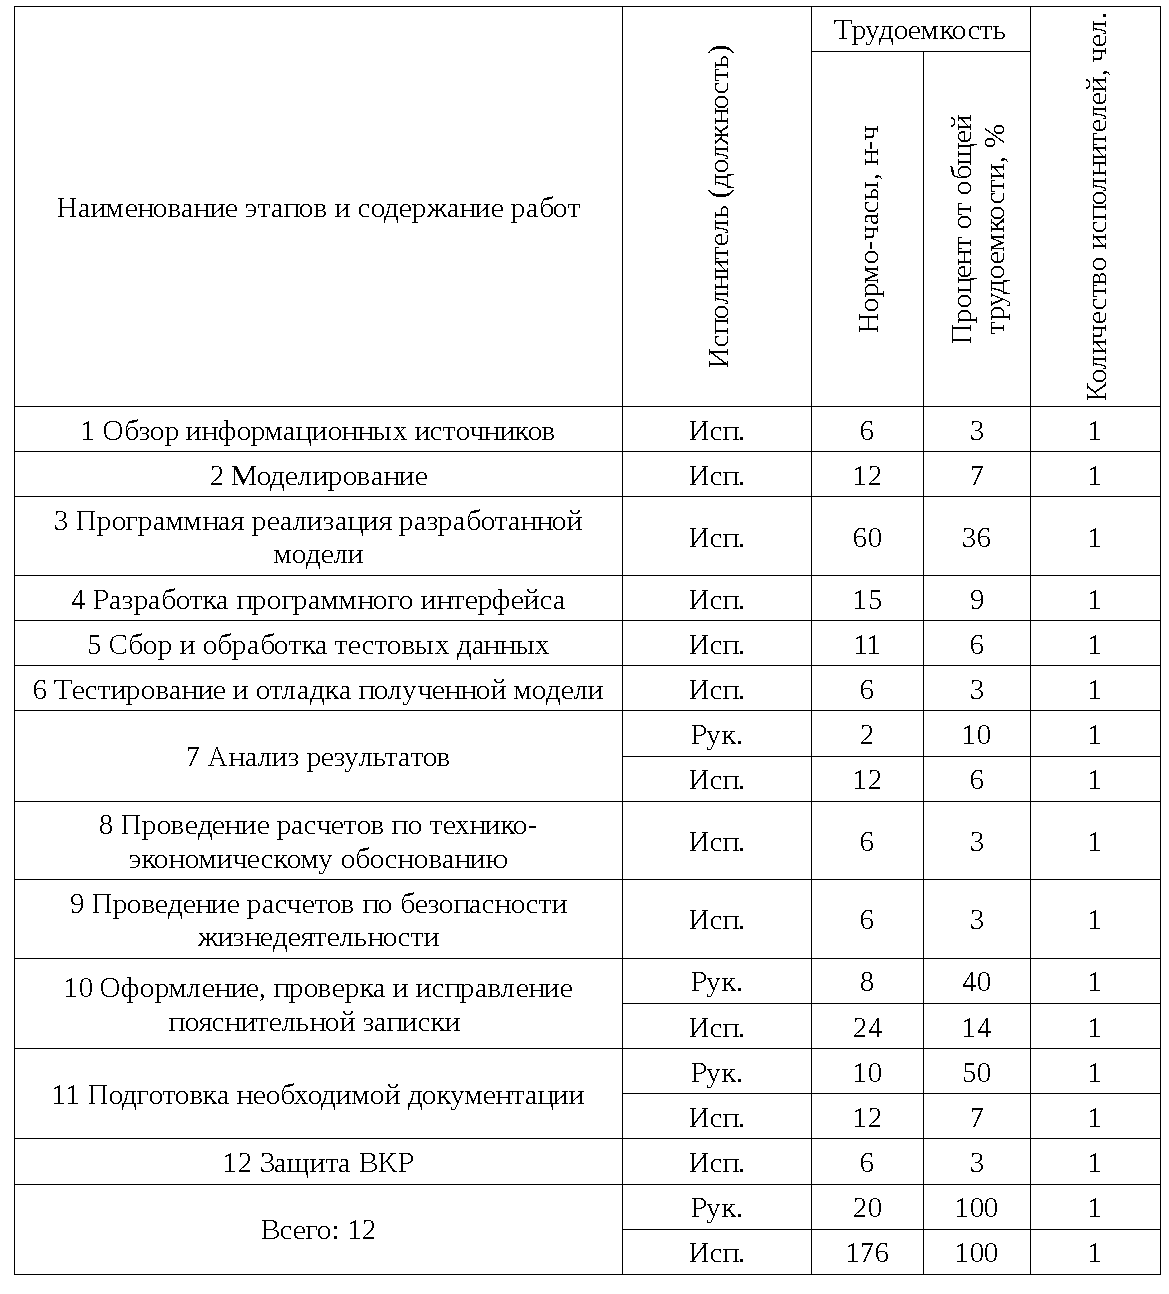
\includegraphics[page=1, width=1\linewidth]{tables/economics/schedule.pdf}
\label{tab:job_is_done_1}
\end{table}


\begin{table}[!ht]
\caption{Диаграмма Ганта}
\centering
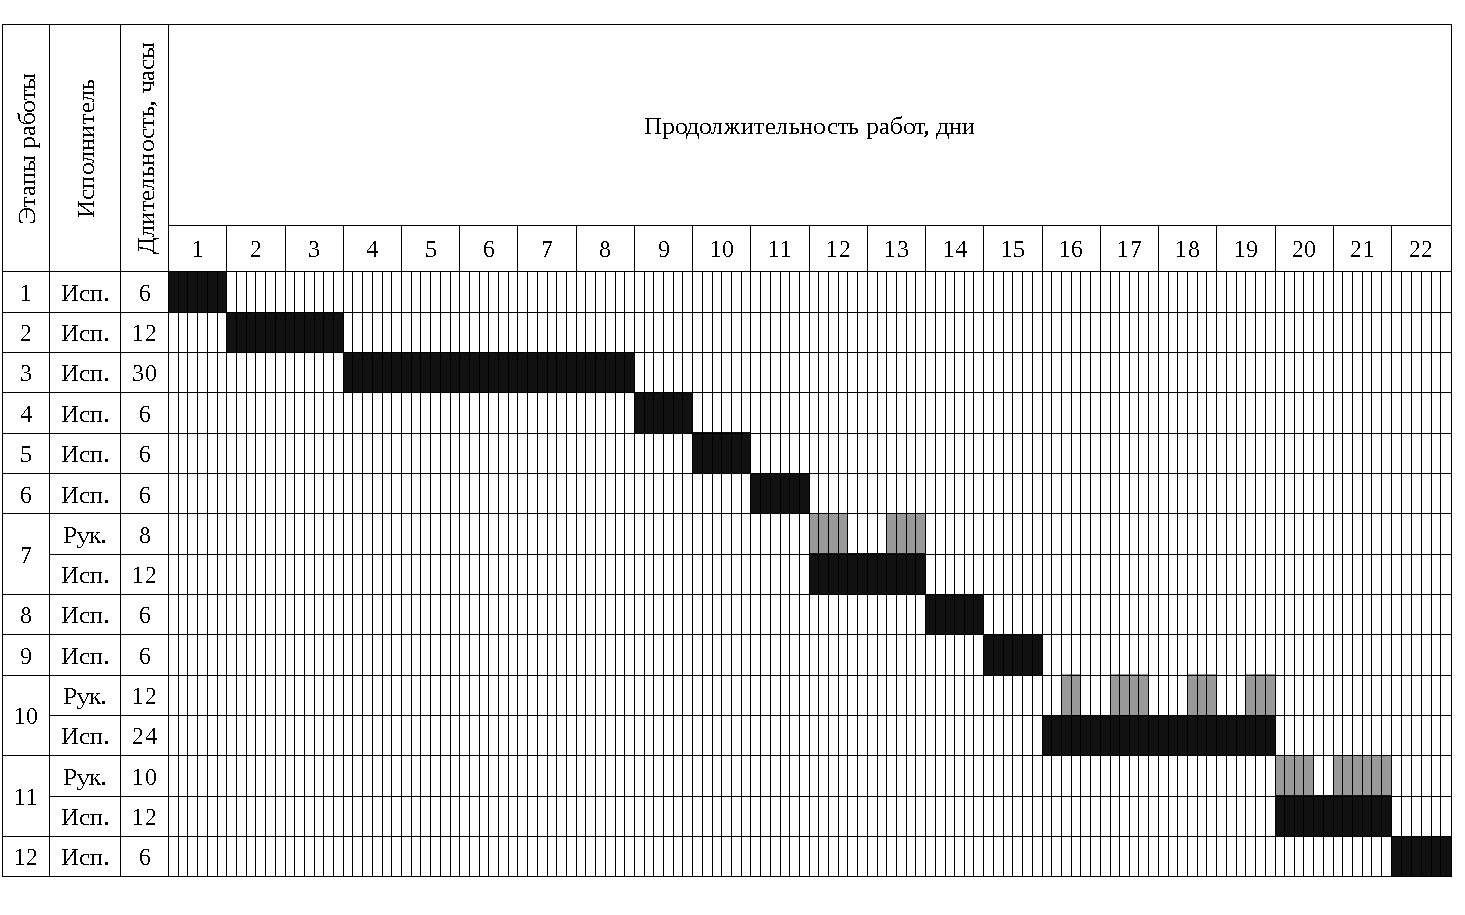
\includegraphics[page=1, width=1\linewidth]{tables/economics/grantt.pdf}
\label{tab:job_is_done_2}
\end{table}

Всего на выполнение проекта руководителем было затрачено 20 часов, исполнителем --- 22 8-часовых
рабочих дня.


\subsection{Определение сметной стоимости проекта}
\subsubsection{Общие положения}

Смета затрат для данной работы состоит из расходов, которые включают в себя следующие статьи:

\begin{itemize}
\item затраты на оборудование и амортизацию;
\item расходы на оплату труда и отчисления на социальные взносы;
\item затраты на основные и вспомогательные материалы;
\item затраты на электроэнергию.
\end{itemize}
\subsubsection{Затраты на оборудование и амортизацию}

Основным оборудованием при проведении работы являются компьютер и принтер, которые 
постановлением Правительства Российской Федерации от 1.01.02 г.~\textnumero~1 отнесены ко второй амортизационной группе – 
<<имущество со сроком полезного использования свыше 2 лет до 3 лет включительно>>~\cite{amort}. 

Определим норму амортизации линейным методом~\cite{frolova}. Расчет производится по формулам:

\begin{center}
 $ N_{a} = \dfrac{1}{T_{n}\times12}\times 100\%,$
 \end{center}
 \begin{center}
 $ A = F_{n}\times N_{a}, $
\end{center}
где~~~~~ \ $N_{a}$ --- месячная норма амортизации;

$T_{n}$ --- срок полезного использования объекта основных средств;

$F_{n}$ --- первоначальная стоимость объекта основных средств;

$A$ --- сумма амортизации за месяц.

Месячная норма амортизации и для ноутбука, и для принтера с учетом трехлетнего срока 
использования объектов основных средств составит:
\begin{center}
$ N_{a} = \dfrac{1}{3\times12}\times 100\% \approx 2,8\%.$\\
\end{center}

Результаты расчётов амортизационных отчислений приведены в таблице \ref{tab:job_is_done_4}.

\begin{table}[!ht]
\caption{Смета затрат на оборудование}
\centering
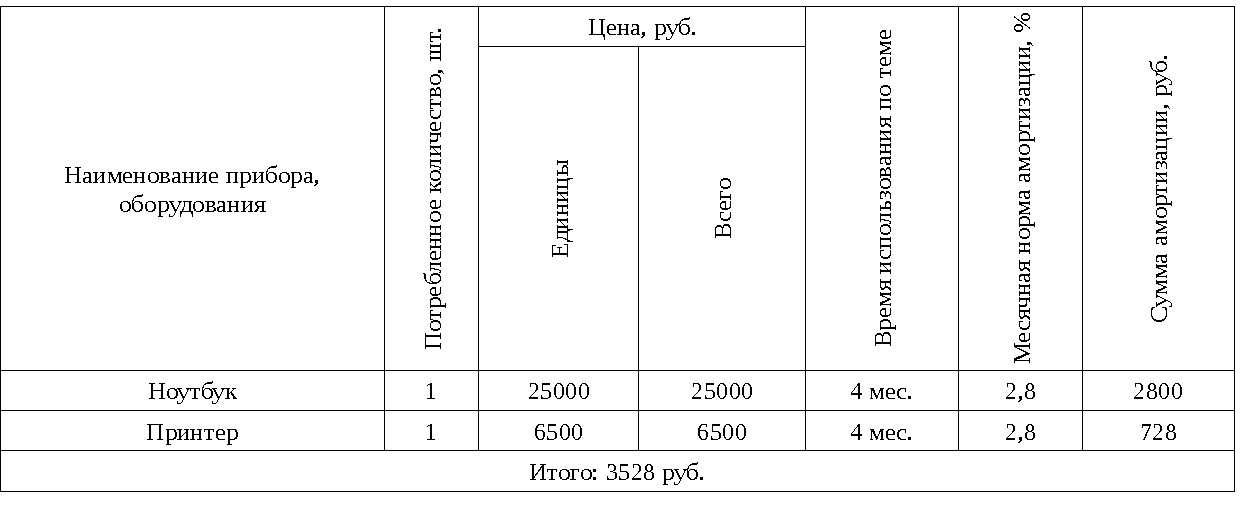
\includegraphics[page=1, width=1\linewidth]{tables/economics/schedule_4.pdf}
\label{tab:job_is_done_4}
\end{table}

\subsubsection{Расходы на оплату труда и социальные взносы}

Статья затрат учитывает выплаты по заработной плате за выполненную работу, 
вычисленные на основании тарифных ставок и должностных окладов в соответствии с принятой в 
организации-разработчике системой оплаты труда. В этой статье также отражаются премии, надбавки и доплаты за 
условия труда, оплата ежегодных отпусков, выплата районного коэффициента и некоторые другие расходы. 
Отчисления на социальные нужды учитывают страховые взносы.

Актуальные для начисления в ПФР на обязательное пенсионное страхование
в 2017 году страховых взносов ставки с выплат работников 
(ст. 426 НК РФ в редакции, действующая с 01.01.2017) составляют 30,2\%.

Результаты расчёта расходов на оплату труда участников проекта представлены в таблице~\ref{tab:job_is_done_5}.

\begin{table}[!ht]
\caption{Расчет расходов на оплату труда участников проекта}
\centering
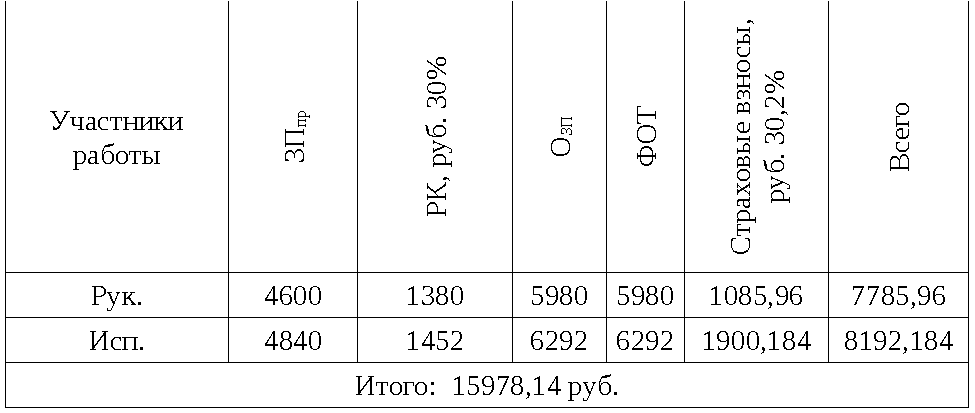
\includegraphics[page=1, width=1\linewidth]{tables/economics/schedule_5.pdf}
\label{tab:job_is_done_5}
\end{table}


\subsubsection{Затраты на основные и вспомогательные материалы}

Статья включает расходы по приобретению и доставке основных и вспомогательных материалов, необходимых для опытно-экспериментальной проработки 
решения, для изготовления макета или опытного оборудования. Сюда включаются и стоимость необходимых материалов для изготовления образцов и 
макетов, и материалов необходимых для оформления требуемой документации.

Результаты расчёта стоимости материалов представлены в \ref{tab:eco_6}.

\begin{table}[!ht]
\caption{Расчёт затрат на основные и вспомогательные материалы}
\centering
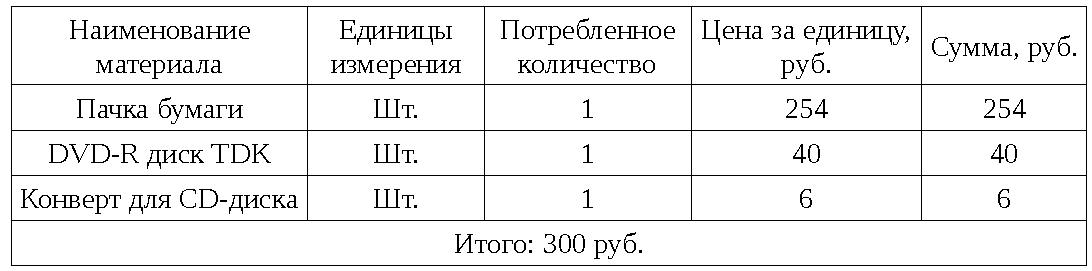
\includegraphics[page=1, width=1\linewidth]{tables/economics/econom.pdf}
\label{tab:eco_6}
\end{table}


\subsubsection{Расходы на электроэнергию}

Статья включает затраты по электроэнергии на технологические нужды. В настоящее время одноставочный
тариф на электроэнергию для населения, проживающего в городских населенных
пунктах Томской области в домах, оборудованных в установленном порядке электрическими 
плитами и (или) электроотопительными приборами,
составляет 2,17 руб./ кВт ч. Тариф введен 
приказом от 23.12.2016 г. \textnumero~6-840 <<О тарифах на электрическую энергию для населения и 
потребителей, приравненных к категории население по Томской области на 2017 год>>~\cite{electr}, 
принятый департаментом тарифного регулирования Томской области.

Результаты расчётов приведены в \ref{tab:eco_7}.

\begin{table}[ht!]
\caption{Затраты на электроэнергию}
\centering
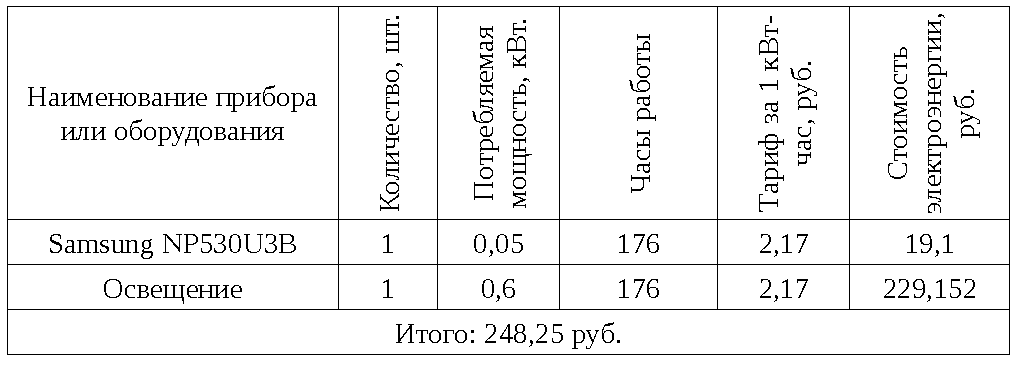
\includegraphics[page=1, width=1\linewidth]{tables/economics/econom_2.pdf}
\label{tab:eco_7}
\end{table}


\subsubsection{Накладные расходы}

Результаты расчёта накладных расходов приведены в таблице~\ref{tab:eco_8}.

\begin{table}[ht!]
\caption{Накладные расходы}
\centering
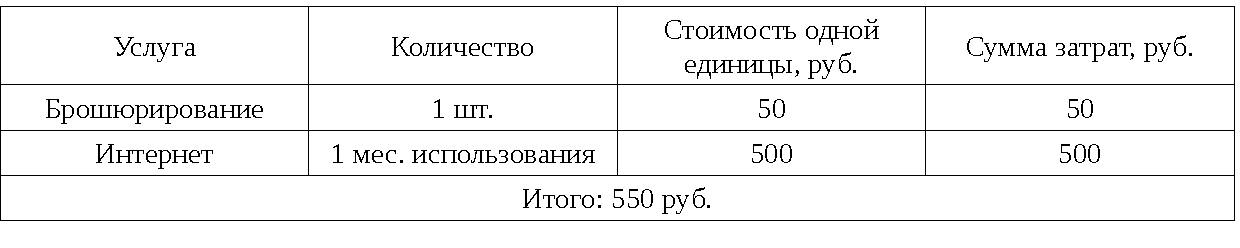
\includegraphics[page=1, width=1\linewidth]{tables/economics/econom_3.pdf}
\label{tab:eco_8}
\end{table}


\subsubsection{Сводная смета затрат}

На основании всех произведённых расчётов составим сводную смету затрат на выполнение работы в виде таблицы \ref{tab:eco_9}.

\begin{table}[ht!]
\caption{Сводная смета затрат}
\centering
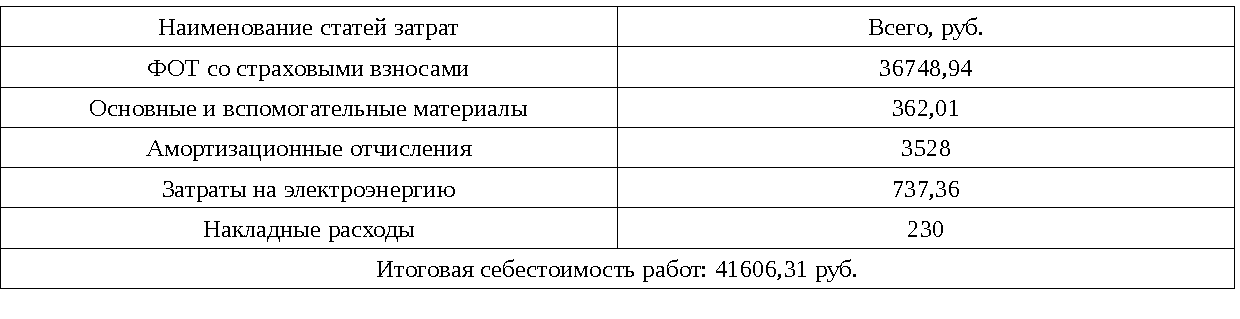
\includegraphics[page=1, width=1\linewidth]{tables/economics/econom_4.pdf}
\label{tab:eco_9}
\end{table}


% \subsection{Научно-технический эффект}
% Количественная оценка научно-технического уровня может быть произведена путём расчёта результативности участников разработки по формуле:
% $$K_{\textit{ну}} = \sum_{i=1}^{n}(K_{\textit{ду}}\cdot d_{i}),$$
% где~~~~~\ $K_\textit{ну}$ – коэффициент научного или научно-технического уровня;
% 
% $K_\textit{дуi}$ – коэффициент достигнутого уровня $\textit{i}{}$-го фактора;
% 
% $d_{i}$ – значимость $i$-го фактора;
% 
% $\textit{n}$ – количество факторов.
% 
% Весовые коэффициенты \textit{d} для каждого из факторов устанавливались экспертным путём. При этом сумма коэффициентов значимости по всем факторам равна единице. Коэффициенты достигнутого уровня факторов также установлены экспертным путём.
% 
% \begin{table}[!ht]
% \caption{Оценка научно-технического уровня разработки}
% \centering
% 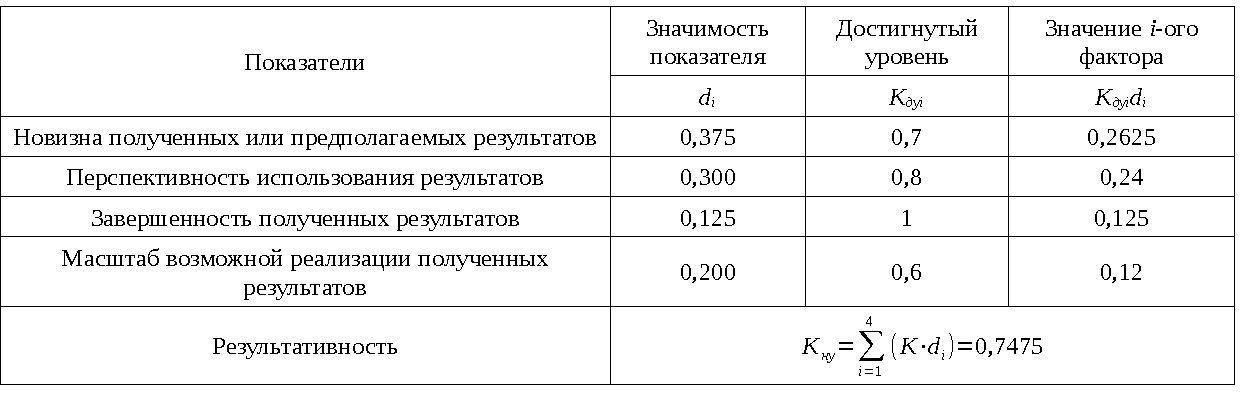
\includegraphics[page=1, width=1\linewidth]{tables/economics/econom_5.pdf}
% \label{tab:eco_10}
% \end{table}

% Рассчитанный коэффициент научно-технической результативности равен 0,7475. Полученное значение достаточно высоко, что говорит об эффективности проведённых работ выше среднего, однако отмечается необходимость дальнейшего развития проекта для достижения завершённости полученных результатов.
% 
% \end{document}